\documentclass[beamer]{standalone}

\usepackage{tikz}

\usetikzlibrary{backgrounds}

\definecolor{almost-white}{HTML}{fefefe}

\begin{document}


\begin{standaloneframe}
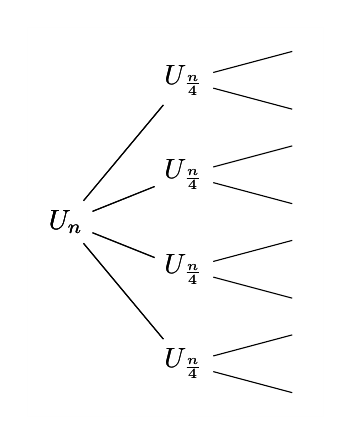
\begin{tikzpicture}[
    grow=right,
    level 1/.style={
        sibling distance=1.2cm,
    },
    level 2/.style={
        sibling distance=.8cm,
    },
    background rectangle/.style={ draw=almost-white, line width=0pt, },
    show background rectangle,
]

\onslide<1>{
    \node {\(U_n\)};
}

\onslide<2>{
    \node {\(U_n\)}
        child foreach \l in {1,2,3,4}
        { node {\(U_{\frac{n}{4}}\)} }
        ;
}

\onslide<3>{
    \node {\(U_n\)}
        child foreach \l in {1,2,3,4}
        { node {\(U_{\frac{n}{4}}\)}
            child foreach \l in {1,2}
            { node {} }
        }
        ;
}

\end{tikzpicture}

\end{standaloneframe}

\end{document}
